%=====================================================================
\section{Flow and tilt of the wall defects in circles}\label{sec:cflow}
Flow fields every 1000 steps (100 time units) on all seeds; methods in Secs.~\ref{sec:md-flow} and \ref{sec:md-tilt}.
\begin{figure}[H]\centering
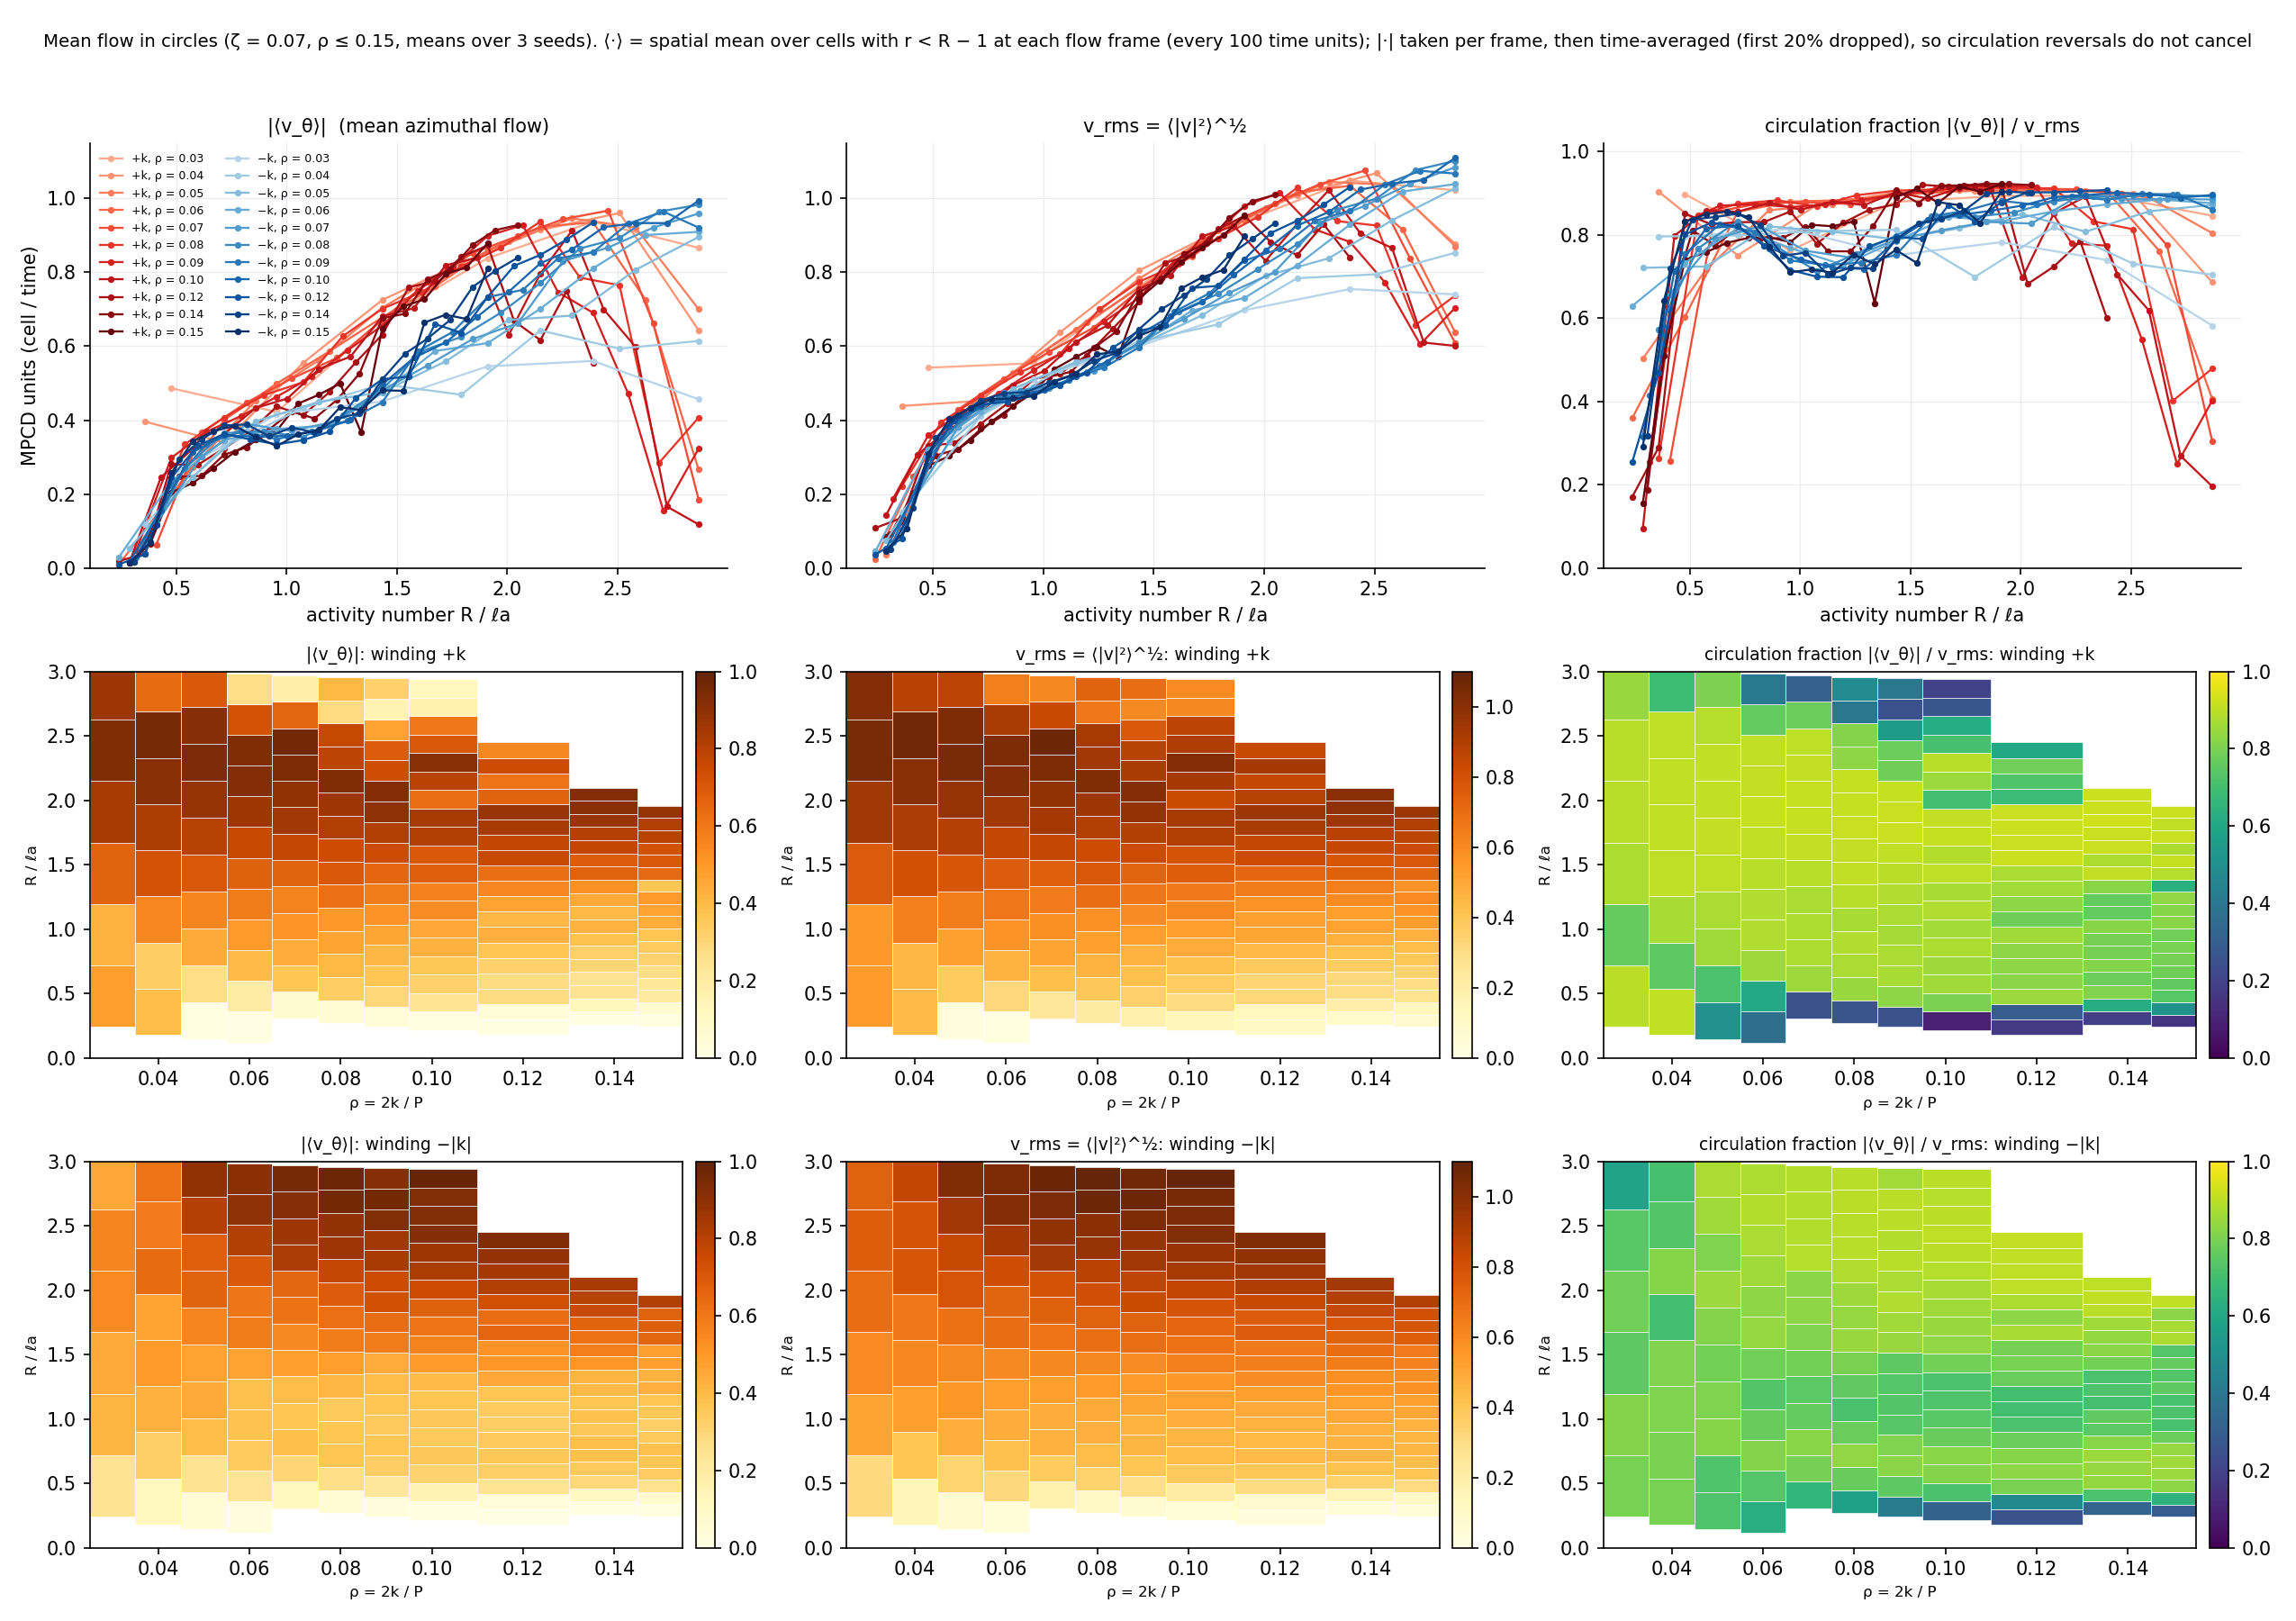
\includegraphics[width=\textwidth]{flow_mean.png}
\caption{Mean flow in circles: $|\langle v_\theta\rangle|$ (spatial mean of the azimuthal velocity per frame, absolute value,
then time-averaged), $v_\mathrm{rms}$ and the circulation fraction $|\langle v_\theta\rangle|/v_\mathrm{rms}$; curves against
$R/\la$ (red $+k$, blue $-|k|$, one per $\rho$) and maps.}\label{fig:flow}
\end{figure}
\begin{figure}[H]\centering
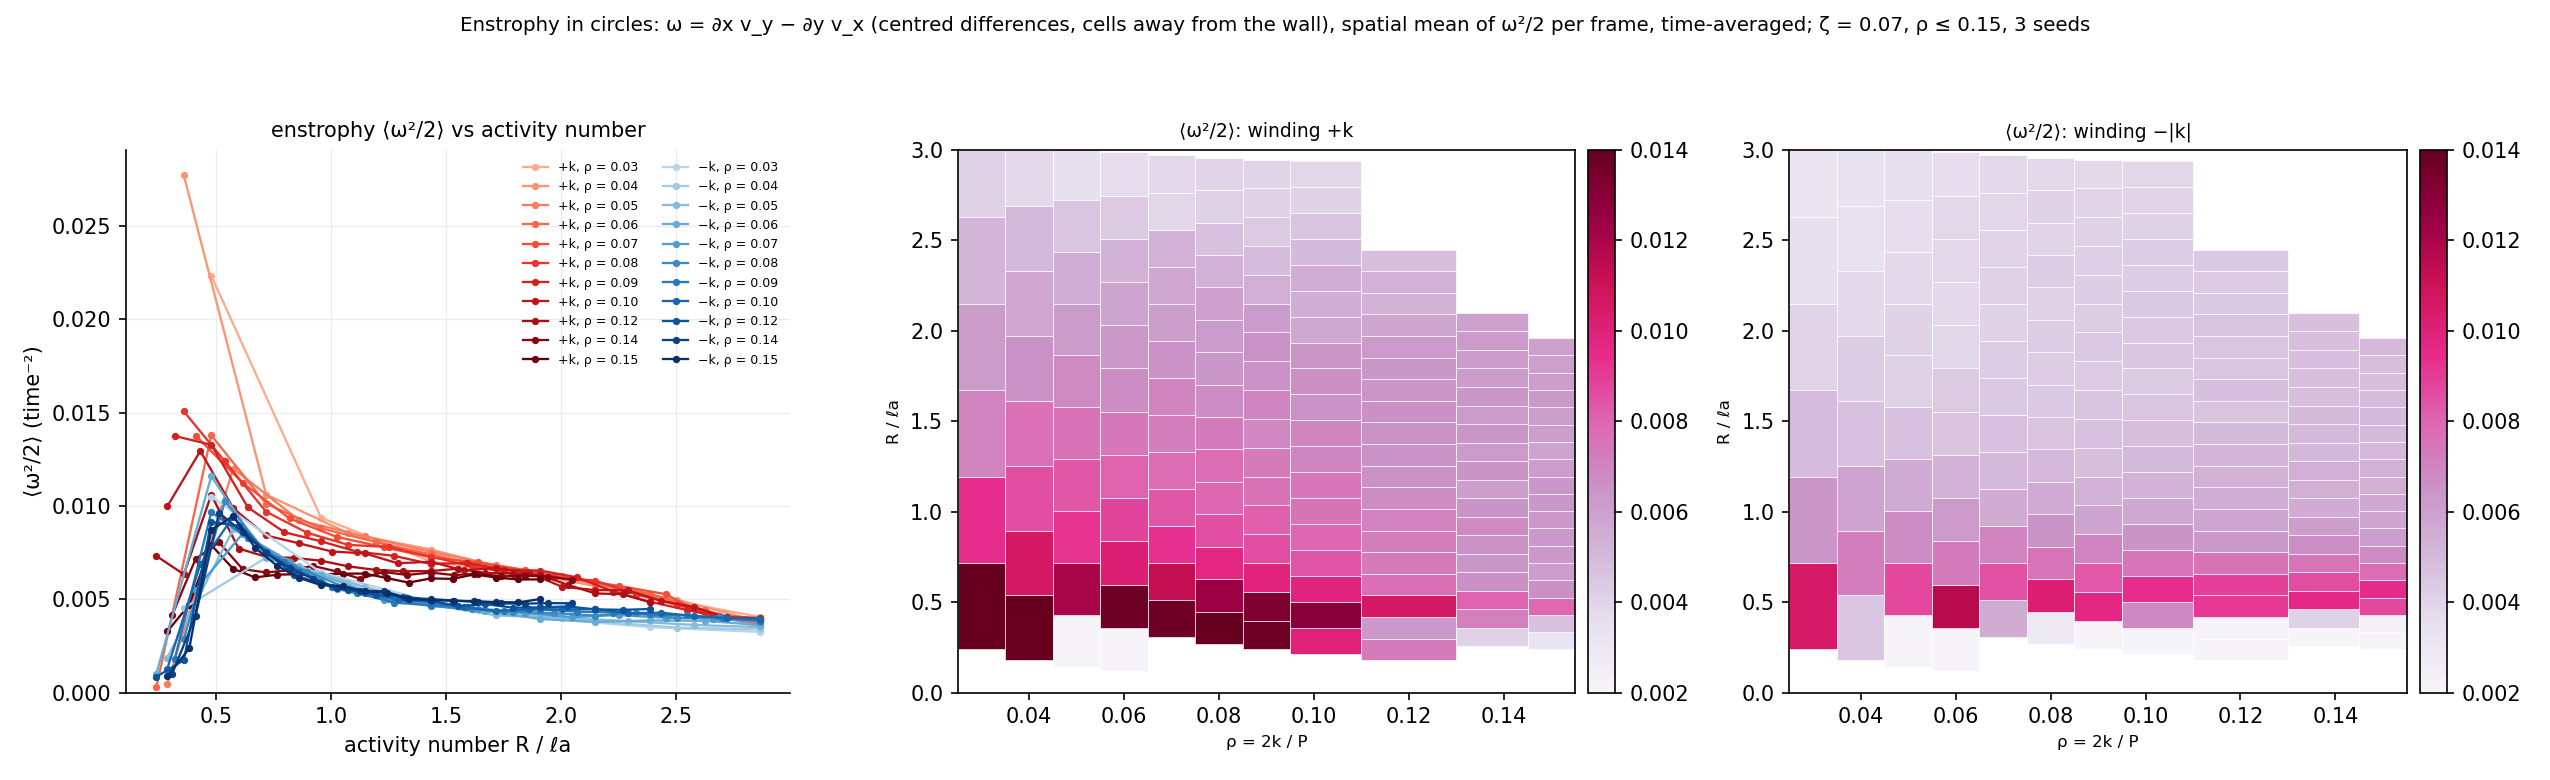
\includegraphics[width=0.9\textwidth]{flow_enstrophy.png}
\caption{Enstrophy $\langle\omega^2/2\rangle$ over interior cells.}\label{fig:enst}
\end{figure}
\begin{figure}[H]\centering
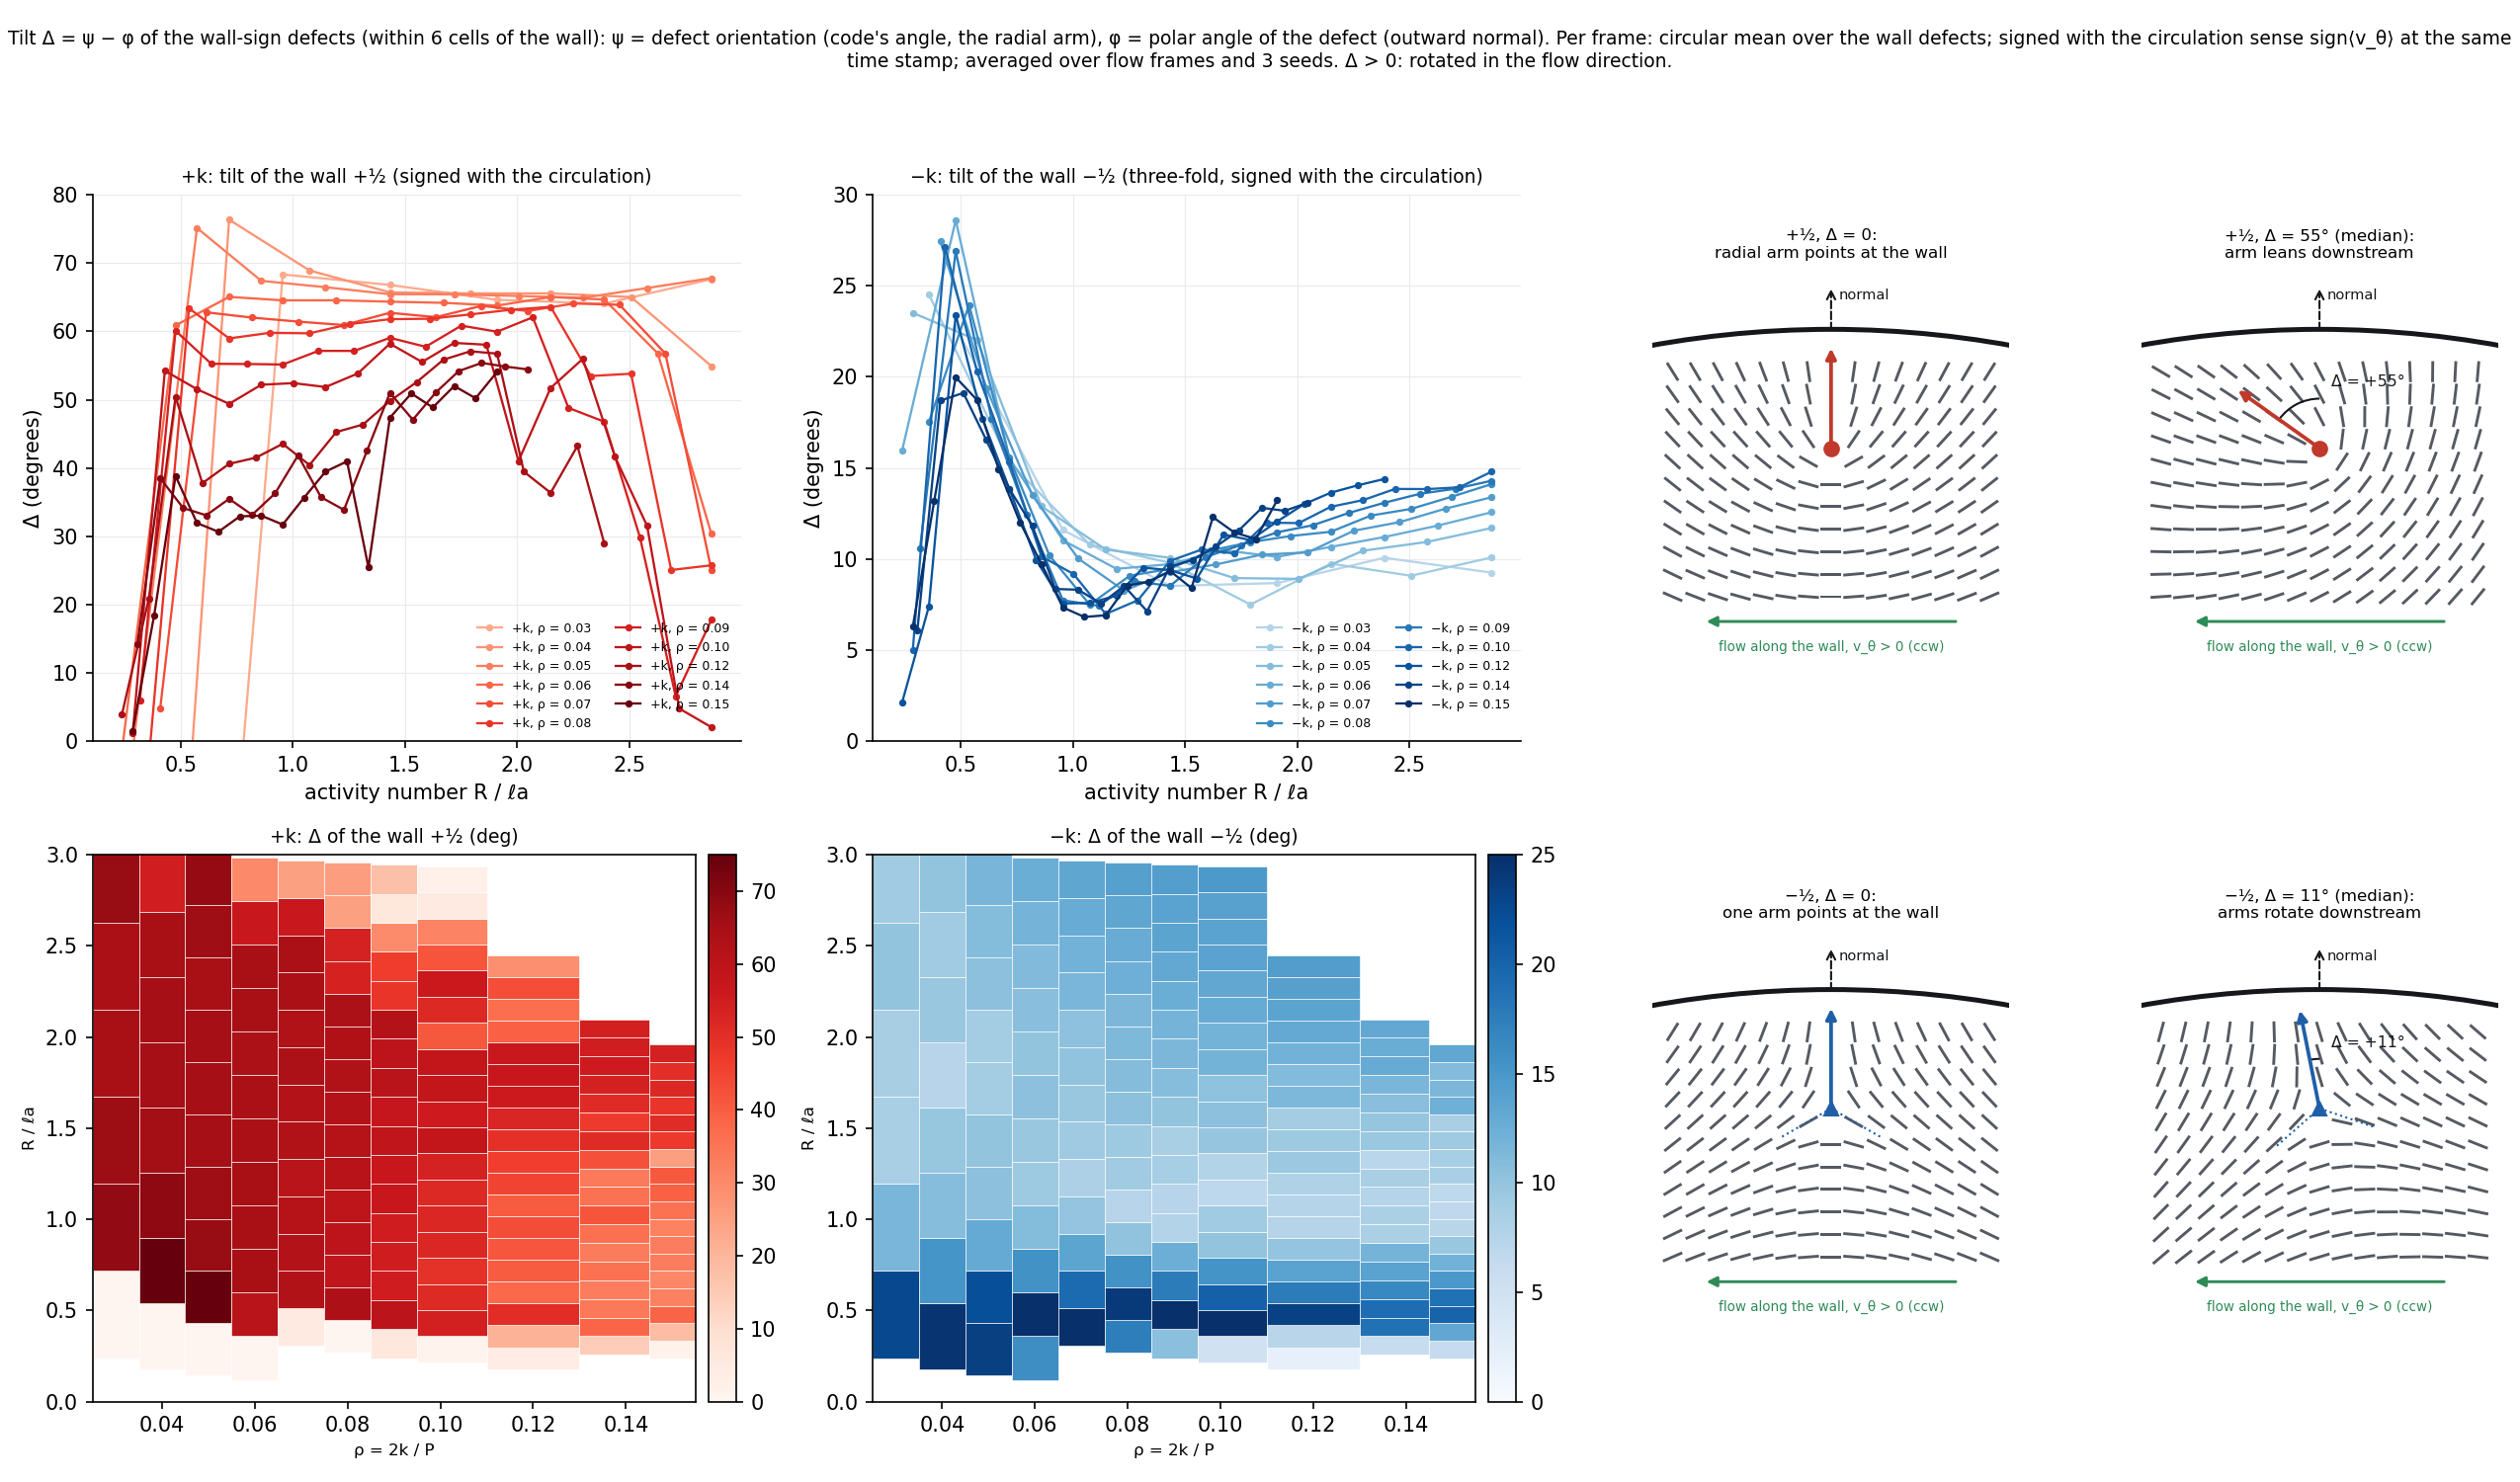
\includegraphics[width=\textwidth]{flow_tilt.png}
\caption{Tilt $\Delta=\psi-\varphi$ of the wall defects (orientation minus polar angle), signed with the circulation sense:
$+\half$ (left) and the three-fold $-\half$ (middle), with schematics (right).}\label{fig:tilt}
\end{figure}
\begin{itemize}
  \item \textbf{Circulation collapses on $R/\la$} for all $\rho$: $|\langle v_\theta\rangle|\approx0.35$ at $0.6\,\la$, 0.9--1.0
        at 2--2.5\,$\la$ (Mach $\sim1$). Circulation fraction 0.8--0.9 between 0.5 and 2.5\,$\la$; below 0.4\,$\la$ no coherent vortex
        ($k=2$: reversals, sign agreement $\approx0.5$). $+k$ circulates slightly faster than $-k$ at 1--2\,$\la$.
  \item \textbf{The vortex breaks down where the layer goes:} for $+k$ the circulation fraction falls from 0.9 to 0.2--0.4 at
        $R\gtrsim2.5\,\la$, with reversals --- the same size where the knee disappears (Table~\ref{tab:sweep}).
  \item \textbf{Enstrophy} peaks ($\approx0.01$--0.015) at 0.4--0.5\,$\la$ and decays to 0.004 at 2.9\,$\la$; $+k$ exceeds $-k$ by
        20--30\% below 2\,$\la$.
  \item \textbf{Tilt:} wall $+\half$ lean downstream by 60--65$^\circ$ at $\rho\le0.06$, decreasing to 30--40$^\circ$ at
        $\rho=0.14$--0.15 (crowded wall); the tilt vanishes where the layer is lost ($R\gtrsim2.5\,\la$) and below 0.4\,$\la$. Wall
        $-\half$ lean downstream by 8--15$^\circ$ (peak $\approx25^\circ$ at 0.5\,$\la$). The sign agrees with the circulation in
        $\approx100\%$ of frames inside the layer window.
  \item \textbf{H4} (the $+1$ bulk appears with circulation) is consistent but untested as a cause: wherever the layer exists the
        vortex exists too, and both disappear together at large $R$. The activity onset ($\zeta=0.05$, $k=9$--10) is the one case
        where the vortex fails at fixed $R/\la$ (Sec.~\ref{sec:activity}); there the bulk charge also drifts above 1.
\end{itemize}
